\documentclass[addpoints]{exam}

\usepackage{amsmath}
\usepackage{amssymb}
\usepackage{enumitem}
\usepackage{graphicx}
\usepackage{hyperref}
\usepackage{multicol}
\usepackage{tikz}
\usepackage{titling}

% Header and footer.
\pagestyle{headandfoot}
\runningheadrule
\runningfootrule
\runningheader{CS 113 Spring 201}{HW 4: Functions, Induction, Graphs}{\theauthor}
\runningfooter{}{Page \thepage\ of \numpages}{}
\firstpageheader{}{}{}

\boxedpoints
\printanswers

\newcommand\union\cup
\newcommand\interx\cap

\graphicspath{{images/}}

\title{Homework 4: Functions, Induction, Graphs}
\author{upper-bound}  % replace with your team name
\date{CS/MATH 113 Discrete Mathematics\\Habib University, Spring 2022}

\begin{document}
\maketitle

\begin{questions}

  \section*{Functions}
  
\question[5] Consider these functions from the set of students in a discrete mathematics class. Under what conditions is the
  function one-to-one if it assigns to every student,
  
  \begin{enumerate}[label=\alph*)]
  \item their mobile phone number.
    \begin{solution}
    \end{solution}
  \item their student identification number.
    \begin{solution}
    \end{solution}
  \item their final grade in the class.
    \begin{solution}
    \end{solution}
  \item their home town.
    \begin{solution}
    \end{solution}
  \item their Ehsas hour appointment.
    \begin{solution}
    \end{solution}
  \end{enumerate}


\question[5] If $f$ and $f \circ g$ are one-to-one, does it follow that $g$ is one-to-one? Justify your answer.
  \begin{solution}
  \end{solution}

\question[5] Prove that a strictly decreasing function from $\mathbb{R}$ to itself is one-to-one. Give an example of a decreasing function from $\mathbb{R}$ to itself that is not one-to-one.
  \begin{solution}
  \end{solution}
  
  \section*{Graphs}
  
\question To lift the spirits of the students on their return, Habib University has decided to build 4 new courtyards--Nature, Ice, Light, and Darkness. Designs are invited and bids are received for the courtyards from 4 architect firms as follows. Parveen Prime can design Nature, Light, and Darkness; Queen Quratulain can design Ice and Light; Reena Rani can design Light and Darkness; and Super Sonam can design Nature and Ice.
  \begin{parts}
  \part[5] Use a bipartite graph to model the four architects and the courtyards that they can design.
    \begin{solution}
    \end{solution}
    
  \part[5] Use Hall’s theorem to determine whether there is an assignment of architects to courtyards so that each architect is assigned one courtyard to design.
    \begin{solution}
    \end{solution}

  \part[5] Provide the assignment, if it exists, of architects to courtyards such that each architect is assigned to a courtyard that she can design.
    \begin{solution}
    \end{solution}
  \end{parts}
  
\question  The simple graphs $G_1 = (V_1,E_1)$ and $G_2 = (V_2,E_2$) are \textit{isomorphic} if there exists a one-to-one and onto function $f$ from $V_1$ to $V_2$ with the property that $a$ and $b$ are adjacent in $G_1$ if and only if $f(a)$ and $f(b)$ are adjacent in $G_2$, for all $a$ and $b$ in $V_1$. Such a function $f$ is called an \textit{isomorphism}. Two simple graphs that are not isomorphic are called \textit{non-isomorphic}.

  In other words, when two simple graphs are isomorphic, there is a one-to-one correspondence between the vertices of the two graphs that preserves the adjacency relationship. Isomorphism of simple graphs is an equivalence relation.

  Determine which of the following pairs of graphs are isomorphic. For each pair of graphs, provide an isomorphism (a bijection between the vertices of the graphs) or a rigorous argument that no such bijection exists.

  \begin{tabular}{cccc}
    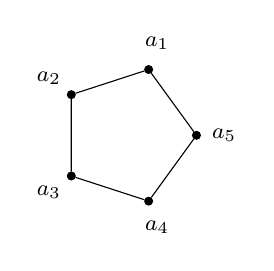
\begin{tikzpicture}
      \tikzstyle{node} = [draw,circle,fill=black,inner sep=1pt]
      \foreach \a in {1,2,...,5}{
        \draw (\a*360/5: 25pt) node(\a)[node]{};
        \draw (\a*360/5: 35pt) node{\footnotesize $a_\a$};
      }
      \path[draw] (1) -- (2) -- (3) -- (4) -- (5) -- (1);
    \end{tikzpicture}
    &
      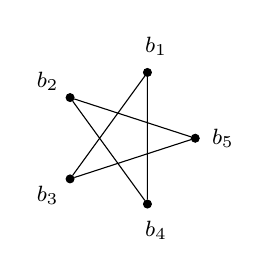
\begin{tikzpicture}
        \tikzstyle{node} = [draw,circle,fill=black,inner sep=1pt]
        \foreach \a in {1,2,...,5}{
          \draw (\a*360/5: 25pt) node(\a)[node]{};
          \draw (\a*360/5: 35pt) node{\footnotesize $b_\a$};
        }
        \path[draw] (2) -- (5) -- (3) -- (1) -- (4) -- (2);
      \end{tikzpicture}
    &
      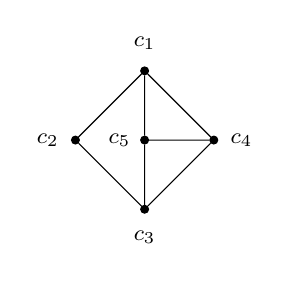
\begin{tikzpicture}
        \tikzstyle{node} = [draw,circle,fill=black,inner sep=1pt]
        \foreach \a in {1,2,...,4}{
          \draw (\a*360/4: 25pt) node(\a)[node]{};
          \draw (\a*360/4: 35pt) node{\footnotesize $c_\a$};
        }
        \node [node, label = left:\footnotesize $c_5$] (5) at (0,0) {};
        \path[draw] (1) -- (2) -- (3) -- (4) -- (1) -- (5) -- (4) -- (3) -- (5);
      \end{tikzpicture}
    &
      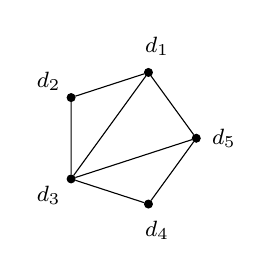
\begin{tikzpicture}
        \tikzstyle{node} = [draw,circle,fill=black,inner sep=1pt]
        \foreach \a in {1,2,...,5}{
          \draw (\a*360/5: 25pt) node(\a)[node]{};
          \draw (\a*360/5: 35pt) node{\footnotesize $d_\a$};
        }
        \path[draw] (1) -- (2) -- (3) -- (4) -- (5) -- (1) -- (3) -- (5);
      \end{tikzpicture}\\
    Graph A & Graph B & Graph C & Graph D    
  \end{tabular}    

  \begin{parts}
  \part[5] Graph A and Graph B
    \begin{solution}
    \end{solution}

  \part[5] Graph A and Graph C
    \begin{solution}
    \end{solution}
    
  \part[5] Graph A and Graph D
    \begin{solution}
    \end{solution}
    
  \part[5] Graph B and Graph C
    \begin{solution}
    \end{solution}
    
  \part[5] Graph B and Graph D
    \begin{solution}
    \end{solution}
    
  \part[5] Graph C and Graph D
    \begin{solution}
    \end{solution}
  \end{parts}

\question[5] Show that in a simple graph with at least two vertices there must be two vertices that have the same degree.
  \begin{solution}
  \end{solution}
  
\question[5] The \textit{complementary graph} $\overline{G}$ of a simple graph $G$ has the same vertices as  $G$. Two vertices are adjacent in $\overline{G}$ if and only if they are not adjacent in $G$. Given $G$ with $v$ vertices and $e$ edges, how many edges are there in $\overline{G}$? Justify your answer.
  \begin{solution}
  \end{solution}
  
  \section*{Induction}
  
\question Prove the following using induction.
  \begin{parts}
  \part[5] Given a a relation $R$ that is reflexive and transitive, $R^n = R$ for all positive integers $n$.
    \begin{solution}
      % Write your solution here
    \end{solution}

  \part[5] A relation $R$ on a set $A$ is transitive if and only if $R^n \subseteq R$ for all positive integers $n$.
    \begin{solution}
      % Write your solution here
    \end{solution}
  \end{parts}


\question[5] Prove via induction that a complete graph with $n$ vertices contains $\dfrac{n(n-1)}{2}$ edges.
  \begin{solution}
  \end{solution}
  
\end{questions}
\end{document}


%%% Local Variables:
%%% mode: latex
%%% TeX-master: t
%%% End:
